\documentclass[12pt, twoside]{article}
\input{../preamble}
\usepackage{float}

\title{Physics}
\author{Chris Huson}
\date{May 2026}

\fancyhead[LE]{\thepage}
\fancyhead[RO]{\thepage \\ First \& last name: \hspace{2.25cm} \,\\  \,}
\fancyhead[LO]{La Scuola d'Italia / Huson / Physics \\* 18 May 2026}

\begin{document}

\subsubsection*{Problem Set: Vectors, Trigonometry, and Frames of Reference}

\begin{enumerate}

\item A force $\vec{F}$ of magnitude $50\,\text{N}$ is directed at $37^\circ$ above the horizontal, as shown.\vspace{0.25cm}
\begin{multicols}{2}
  \begin{enumerate}[itemsep=1cm]
    \item Find the horizontal component $F_x$.
    \item Find the vertical component $F_y$.\vspace{1.5cm}
  \end{enumerate}
  \begin{flushright}
    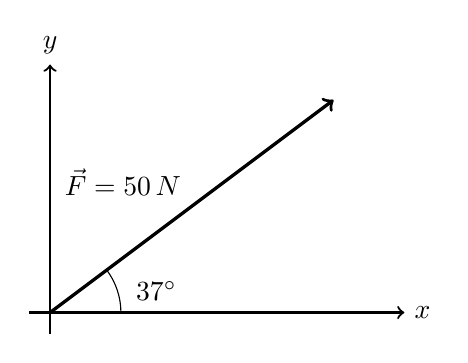
\begin{tikzpicture}[scale=0.9]
      \draw[->, thick] (-0.3,0)--(5,0) node[right]{$x$};
      \draw[->, thick] (0,-0.3)--(0,3.5) node[above]{$y$};
      \draw[->, very thick] (0,0)--(4,3) node[midway, above left]{$\vec{F}=50\,\text{N}$};
      \draw (1,0) arc [start angle=0, end angle=37, radius=1];
      \node at (1.5,0.3){$37^\circ$};
    \end{tikzpicture}
  \end{flushright}
\end{multicols}\vspace{2cm}

\item A car's velocity has components $v_x = 12\,\text{m/s}$ (east) and $v_y = 5\,\text{m/s}$ (north).\vspace{0.25cm}
\begin{multicols}{2}
  \begin{enumerate}[itemsep=1cm]
    \item Find the speed $|\vec{v}|$.
    \item Find the direction $\theta$, measured north of east, to the \emph{nearest degree}.\vspace{1.5cm}
  \end{enumerate}
  \begin{flushright}
    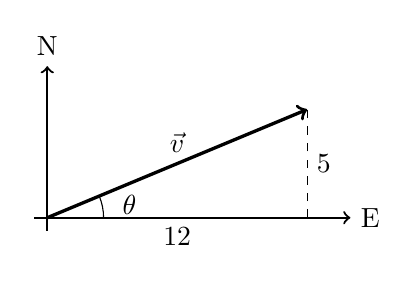
\begin{tikzpicture}[scale=0.55]
      \draw[->, thick] (-0.3,0)--(7,0) node[right]{E};
      \draw[->, thick] (0,-0.3)--(0,3.5) node[above]{N};
      \draw[->, very thick] (0,0)--(6,2.5) node[midway, above]{$\vec{v}$};
      \draw[dashed] (6,0)--(6,2.5);
      \node at (6,1.25)[right]{$5$};
      \node at (3,0)[below]{$12$};
      \draw (1.3,0) arc [start angle=0, end angle=22.6, radius=1.3];
      \node at (1.9,0.3){$\theta$};
    \end{tikzpicture}
  \end{flushright}
\end{multicols}\vspace{1cm}

\newpage

\item \textbf{Frame of reference --- on a train.} A train travels east at $25\,\text{m/s}$ relative to the ground. A passenger walks toward the front of the train at $1.5\,\text{m/s}$ relative to the train.
  \begin{enumerate}[itemsep=1.25cm]
    \item What is the passenger's velocity relative to the ground?
    \item A car drives \emph{west} at $15\,\text{m/s}$ relative to the ground. What is the passenger's velocity relative to the car?
    \vspace{0.5cm}
  \end{enumerate}

\item \textbf{Frame of reference --- crossing a river.} A boat heads due north across a river, moving at $4.0\,\text{m/s}$ relative to the water. The river itself flows east at $3.0\,\text{m/s}$ relative to the ground.\vspace{0.25cm}
\begin{multicols}{2}
  \begin{enumerate}[itemsep=0.8cm]
    \item Find the boat's speed relative to the ground.
    \item Find the angle of the boat's motion, measured east of north, to the \emph{nearest degree}.\vspace{1cm}
  \end{enumerate}
  \begin{flushright}
    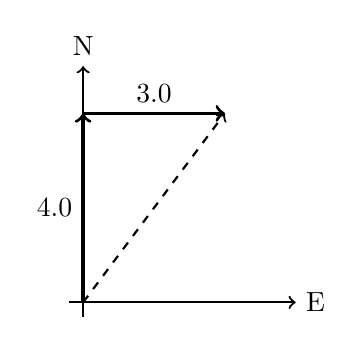
\begin{tikzpicture}[scale=0.6]
      \draw[->, thick] (-0.3,0)--(4.5,0) node[right]{E};
      \draw[->, thick] (0,-0.3)--(0,5) node[above]{N};
      \draw[->, very thick] (0,0)--(0,4) node[midway, left]{$4.0$};
      \draw[->, very thick] (0,4)--(3,4) node[midway, above]{$3.0$};
      \draw[->, thick, dashed] (0,0)--(3,4);
    \end{tikzpicture}
  \end{flushright}
\end{multicols}\vspace{0.5cm}

\item \textbf{Energy unit conversions.} A typical chocolate bar contains about $1.0\times 10^{6}\,\text{J}$ of food energy.
  \begin{enumerate}[itemsep=0.8cm]
    \item Convert this to kilocalories. ($1\,\text{kcal} = 4184\,\text{J}$.)
    \item Convert this to kilowatt-hours. ($1\,\text{kWh} = 3.6\times 10^{6}\,\text{J}$.)
    \item How many electron-volts is $1.0\times 10^{6}\,\text{J}$? ($1\,\text{eV} = 1.6\times 10^{-19}\,\text{J}$.)
  \end{enumerate}

\end{enumerate}
\end{document}
